\addsection{Other Rules}{\images/armorer.png}
\subsection*{\hypertarget{Trading}{Trading}}
The \hyperlink{Trading Post}{trading post field} and other effects allow the players to trade resources with the game in accordance to the table below.
You may also \textbf{remove cards} from your hand at the trading post to gain 1 gold.
\textbf{Note}: Specialty, statistic, starting ability and magic arrows cannot be removed in this way.\par
In \textbf{alliance} and \textbf{co-operative} scenarios, players are allowed to trade resources and cards following these rules:
\begin{itemize}
  \item In alliance scenarios, allies may trade resources freely at any time on their turns except during combat.
  \item In co-operative scenarios, resources may be given to other players when visiting a trading post.
  \item In both scenario types, allies may trade \textbf{spell} and \textbf{artifact} cards in any mix if they have heroes on adjacent fields.
    Only cards from their hands may be traded and you must give and receive an equal amount of cards.
\end{itemize}
\begin{center}
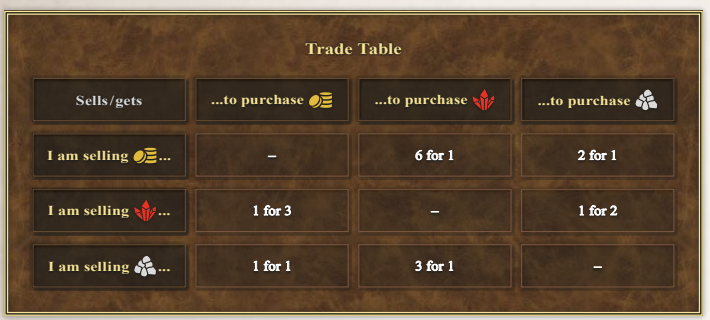
\includegraphics[scale=1]{\images/trade_table.png}
\end{center}

\clearpage

\subsection*{\hypertarget{Difficulty}{Difficulty}}
During set up, players must choose the game’s difficulty.
There are four different difficulties, each with a different starting bonus that players receive during set up:
\begin{itemize}
  \item \textbf{Easy} – Roll 2 \includesvg[height=10px]{\svgs/resource_die.svg} and receive resources from both – OR – Search (2) the artifact deck, twice.
  \item \textbf{Normal} – Roll 2 \includesvg[height=10px]{\svgs/resource_die.svg} and receive the resources from one of them – OR – Search (2) the artifact deck.
  \item \textbf{Hard} – Roll 1 \includesvg[height=10px]{\svgs/resource_die.svg} and receive the resources on it – OR – reveal cards from the top of the artifact deck until you find 1 minor artifact and add it to your hand.
  \item \textbf{Impossible} – No starting bonus.
\end{itemize}
All \textbf{artifacts} received from a starting bonus should be placed into your \textbf{hand} and not shuffled into your starting deck.
Shuffle the artifact deck and its discard pile together afterwards, and then discard one artifact from the top to form the artifact discard pile again.\par
The chosen difficulty also determines the number and type of neutral enemies that are encountered during neutral combat:
\begin{center}
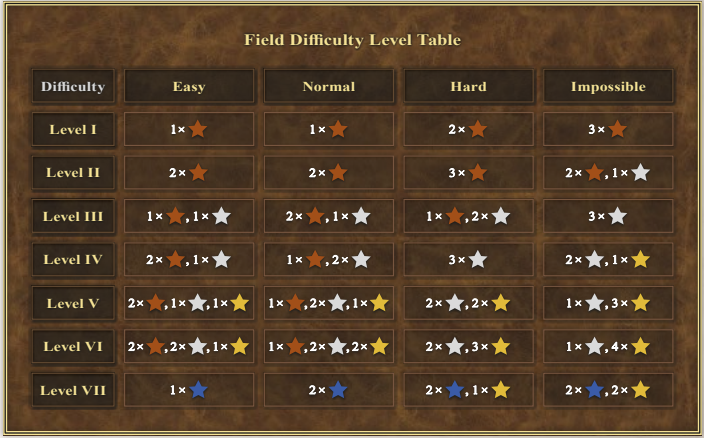
\includegraphics[scale=1]{\images/field_difficulty.png}
\end{center}
